\section{Experimental non-Gaussian measurement computations}
\label{sec:nonGaussian}

Version 0.2 extends the same resource--pattern--execution architecture to pure
non-Gaussian trajectories. The extension is not a universal non-Gaussian
compiler. It provides finite resources, conditional measurements, classical
control and resource-assisted transformations whose mathematical maps can be
tested. The preimplementation audit is recorded in
\texttt{docs/non\_gaussian\_design.md}; the complete tutorial and capability
contract are in \texttt{docs/non\_gaussian.md}.

\subsection{State space, preparation and capabilities}

Piquasso's pure Fock simulator stores the globally truncated space
\begin{align}
 \mathcal H_{d,c}&=\operatorname{span}\{
 |n_1,\ldots,n_d\rangle:\textstyle\sum_jn_j<c\},\\
 D(d,c)&=\binom{d+c-1}{d}.
\end{align}
Thus $c$ is not a per-mode cutoff. For example, two modes at $c=64$ have
$D=2080$ amplitudes. A complex double vector alone requires $16D$ bytes;
density matrices and native gate workspaces can be much larger. Execution
requires an explicit integer cutoff. A configurable dimension guard defaults
to $D\leq10^6$, with a warning from $D=10^5$. This guard bounds the vector
space requested, not peak process memory.

\texttt{FockInput} retains the single-mode normalized-vector interface.
\texttt{FockSuperposition} adds sparse occupation tuples with explicit
amplitudes. Its mode order follows the labels supplied to
\texttt{PrepareResource}, or the ordered input labels when supplied as a
correlated initial state. Shapes, normalization, finiteness, nonnegative integer
occupations, uniqueness and cutoff support are checked. Public native pure
Piquasso amplitudes can be copied into this description; arbitrary mixed
native input is not accepted. Tensor preparation projects onto the global
space and records the retained weight before normalization.

The backend advertises named capabilities through \texttt{supports(feature)}.
The execution preflight rejects non-Gaussian resources or gates on a Gaussian
backend, and rejects unavailable noise/measurement features on the pure-Fock
backend. Gaussian and non-Gaussian commands can be interleaved in a pattern
executed wholly in Fock space. There is no implicit representation switching.
Explicit pure Gaussian inputs are converted to Fock preparations; a mixed
Gaussian covariance requires an unavailable mixed-input implementation.

\subsection{Cats, cubic resources and unitary conventions}

An ideal normalized cat has the form
\begin{equation}
 |C_\epsilon(\alpha)\rangle=
 \frac{|\alpha\rangle+\epsilon|-\alpha\rangle}
 {\sqrt{2(1+\epsilon e^{-2|\alpha|^2})}},\quad \epsilon\in\{-1,1\}.
\end{equation}
Its number coefficients are proportional to
$\alpha^n[1+\epsilon(-1)^n]/\sqrt{n!}$, hence parity is exactly $\epsilon$.
The mean photon number is
\begin{equation}
 \langle n\rangle=|\alpha|^2
 \frac{1-\epsilon e^{-2|\alpha|^2}}
 {1+\epsilon e^{-2|\alpha|^2}}.
\end{equation}
Logarithmic factorials and parity-aware rescaling avoid factorial overflow.
\texttt{CatResource} constructs the projection at the execution cutoff and
monitors its retained infinite-state weight. The older
\texttt{FockInput.cat} instead defines an explicitly normalized finite vector;
a cutoff-dependent factory must rebuild that vector during convergence scans.
The zero-norm odd cat at $\alpha=0$ is rejected.

The nonlinear gate conventions preserve the original adapter and Piquasso:
\begin{align}
 C(\gamma)&=\exp(i\gamma q^3/6), & C^\dagger pC&=p+\gamma q^2,\label{eq:cubicConvention}\\
 K(\kappa)&=\exp(i\kappa n^2), & K|n\rangle&=e^{i\kappa n^2}|n\rangle,\\
 Q(s)&=\exp(isq^2/4), & Q^\dagger pQ&=p+sq.
\end{align}
All angles and coefficients use $\hbar=2$. A desired phase $\exp(i\lambda q^3)$
therefore requires $\gamma=6\lambda$. \texttt{CubicPhaseResource} represents
$C(\gamma)S(-r)|0\rangle$, with finite $r\geq0$. Its untruncated wavefunction is
\begin{equation}
 \phi_{\gamma,r}(q)=\frac{e^{-q^2/(4e^{2r})}}{(2\pi e^{2r})^{1/4}}
 e^{i\gamma q^3/6}.
\end{equation}
Preparing such a resource through a simulated cubic gate is a resource model,
not a proposal for experimentally synthesizing that gate for free.
Ancillary-state approaches to weak cubic nonlinearities and adaptive cubic
measurements motivate this separation~\cite{marek2011,miyata2016}; the implemented
map below is independently derived rather than assumed identical to a specific
experimental circuit.

\subsection{Ideal ladder operations versus heralding}

The mathematical updates \texttt{PhotonSubtract} and \texttt{PhotonAdd} are
\begin{equation}
 |\psi\rangle\longmapsto
 \frac{a|\psi\rangle}{\sqrt{\langle n\rangle}},\qquad
 |\psi\rangle\longmapsto
 \frac{a^\dagger|\psi\rangle}{\sqrt{\langle n\rangle+1}}.
\end{equation}
They apply the occupation factors $\sqrt n$ and $\sqrt{n+1}$. In the inspected
Piquasso 8.0.1 source, \texttt{Create}/\texttt{Annihilate} use unit occupation
shifts; the adapter therefore does not equate those instructions with these
mathematical ladders. The unnormalized squared ladder norm is recorded
separately from truncation weight. It is not a physical success probability:
$a^\dagger$ is not by itself a trace-nonincreasing Kraus operator. A numerically
zero norm ($\leq10^{-28}$) and addition leaving the supported space are errors.

The \texttt{photon\_subtraction} pattern instead couples the input to vacuum
with a beam splitter and counts the tap. Under the beam-splitter convention
used here, the count-$k$ map on an input number state is
\begin{equation}
 M_k|n\rangle=
 \sqrt{\binom nk}(\sin\theta)^k(\cos\theta)^{n-k}|n-k\rangle.
\end{equation}
Consequently
\begin{equation}
 P(k|n)=\binom nk\sin^{2k}\theta\cos^{2(n-k)}\theta.
\end{equation}
Selecting $k=1$ is physical heralded subtraction. Finite tap angle retains an
attenuation factor; the resulting conditional map is not identical to normalized
$a$. No outcome is silently postselected, and the simulator does not interpret
a selected trajectory as the number of experimental trials until success.

\subsection{Conditional counting and homodyne}

For a joint pure state $\sum_{n,\bm s}A_{n,\bm s}|n\rangle|\bm s\rangle$,
number detection gives
\begin{equation}
 P(n)=\sum_{\bm s}|A_{n,\bm s}|^2,\qquad
 B_{\bm s}=A_{n,\bm s}/\sqrt{P(n)}.
\end{equation}
Sequential destructive detection on multiple modes realizes the joint count
distribution through conditional probabilities. Count records are integers;
expressions such as $(-1)^n$ and polynomial corrections use the existing safe
expression tree and dependency DAG.

Piquasso's inspected pure-Fock homodyne sampler does not return a conditional
state. PhotoGraphiQ adds an explicit wavefunction adapter. Define
\begin{equation}
 h_n(x)=\frac{\operatorname{He}_n(x)e^{-x^2/4}}
 {(2\pi)^{1/4}\sqrt{n!}},
\end{equation}
where $\operatorname{He}_n$ is the probabilists' Hermite polynomial. For
$q_\vartheta=q\cos\vartheta+p\sin\vartheta$,
\begin{align}
 \widetilde B_{\bm s}(x)&=\sum_n A_{n,\bm s}e^{-in\vartheta}h_n(x),\\
 p_\vartheta(x)&=\sum_{\bm s}|\widetilde B_{\bm s}(x)|^2,\\
 B_{\bm s}(x)&=\widetilde B_{\bm s}(x)/\sqrt{p_\vartheta(x)}.
\end{align}
The adapter evaluates $h_n$ by its normalized three-term recurrence. The
projection is exact within the stored finite expansion. Sampling numerically
integrates this nonnegative marginal and inverts its CDF. Absolute and relative
quadrature tolerances are $10^{-10}$, root tolerance is $10^{-10}$, and the
interval $[-2\sqrt c-10,2\sqrt c+10]$ must capture unit mass within $10^{-7}$.
Failed integration and zero-density postselection are explicit errors.

Fixed measurement outcomes may be supplied for branchwise experiments.
\texttt{measurement\_statistics} distinguishes conditional probability from
probability density and records whether selection was explicit. The sum of
their logarithms is a joint log likelihood. With homodyne this is a density,
not a nonzero probability of an exact real outcome. Finite detector bins require
integration. Noisy Fock homodyne, Fock heterodyne and general mixed measurement
updates remain unavailable. Gaussian likelihood diagnostics have not been added
to the pre-existing moment backend.

\subsection{Finite-resource injection and nonlinear feedforward}

Let $u$ be the input and $a$ the resource mode. The chronological sequence
$R_a(\pi/2)$, $\CZ_{ua}(-1)$, $R_a(-\pi/2)$ realizes inverse SUM:
$q_a\mapsto q_a-q_u$ and $p_u\mapsto p_u+p_a$.
Measuring the resource position at $m$ leaves the unnormalized input wavefunction
\begin{equation}
 \psi(q)\phi(q+m).\label{eq:resourceFilter}
\end{equation}
\texttt{resource\_injection} encodes this sequence. Cat injection supplies
$\phi=C_\epsilon(\alpha)$ and produces a conditional cat-wavefunction filter;
it does not define a deterministic unitary cat gate.

For the cubic resource, expand
$(q+m)^3=q^3+3mq^2+3m^2q+m^3$. The corrections
\begin{equation}
 Q(-2\gamma m),\qquad Z(-\gamma m^2)
\end{equation}
remove the outcome-dependent quadratic and linear phases. Up to global phase,
the output of \texttt{cubic\_injection} is
\begin{equation}
 \psi_{\rm out}(q)\propto
 \psi(q)e^{i\gamma q^3/6}
 \exp\!\left[-\frac{(q+m)^2}{4e^{2r}}\right].\label{eq:cubicFilter}
\end{equation}
The finite envelope remains physical filtering; it cannot be discarded when
reporting gate fidelity. The state remains on the input node, so this is
resource-assisted gate injection rather than relocation of the input state.
Increasing squeezing broadens the envelope while increasing photon-number cost.
The nonlinear correction $m^2$ is an ordinary classical dependency in the IR.

\begin{lstlisting}[language=Python]
pattern = pg.non_gaussian.cubic_injection(
    gamma=0.3, squeezing=0.2)
study = pg.cutoff_convergence(
    pattern, [36, 48, 64],
    measurement_outcomes={"m": 0.4})
state = study.results[-1].state
print(study.rows[-1]["fidelity_to_previous"])
\end{lstlisting}

\subsection{Output analysis and truncation evidence}

Fock snapshots expose pure vectors where available, density matrices, occupation
probabilities, reductions, photon number, parity and quadrature moments. For
one mode, with $\mu=\langle a\rangle$ and $\nu=\langle a^2\rangle$,
\begin{align}
 \langle q_\vartheta\rangle&=2\Re(e^{-i\vartheta}\mu),\\
 \langle q_\vartheta^2\rangle&=2\langle n\rangle+1+
 2\Re(e^{-2i\vartheta}\nu).
\end{align}
The $+1$ term avoids the spurious top-level boundary error obtained by squaring
a quadrature matrix truncated too early. State comparison aligns occupation
tuples, not anonymous vector indices. The implemented fidelity and trace distance
are
\begin{align}
 F(\rho,\sigma)&=\left[\tr\sqrt{\sqrt\rho\sigma\sqrt\rho}\right]^2,\\
 T(\rho,\sigma)&=\tfrac12\|\rho-\sigma\|_1.
\end{align}
When one state is pure, fidelity reduces to $\tr(\rho\sigma)$.
Ordered output labels must agree; differing cutoffs are padded by occupations.

The single-mode Wigner marginal uses analytic displacement matrix elements:
\begin{equation}
 W(q,p)=\frac{1}{2\pi}\tr[\rho D(q+ip)(-1)^n].
\end{equation}
Here $D(\beta)=\exp(\beta a^\dagger-\beta^*a)$ and the phase-space amplitude
is $(q+ip)/2$. The density integrates to one over $dq\,dp$. The finite-grid
negative volume is $\int\max(-W,0)dq\,dp$ over the stated window; captured mass
is reported separately. Window expansion and grid refinement are independent
of Hilbert-space cutoff convergence. Tests include the vacuum and
$W_{|1\rangle}=(q^2+p^2-1)e^{-(q^2+p^2)/2}/(2\pi)$, whose full negative volume
is $2e^{-1/2}-1$.

Every native gate and tensor preparation records retained norm and population
in the last two total-photon shells. A default norm deviation above $10^{-3}$
raises an error. Smaller deviations above $10^{-8}$ warn before normalization;
boundary population above $0.02$ warns independently. These thresholds are
configurable diagnostics, not rigorous error bounds. In particular, the native
cubic instruction exponentiates the cube of a truncated position matrix and
can conserve norm exactly while representing a poorly converged state.

\texttt{cutoff\_convergence} compares adjacent increasing cutoffs and records
norms, boundary populations, moments, fidelity, trace distance, probability
$L^1$ change, dimensions and local times. Differing outcomes mark trajectories
incomparable; using the same seed does not fix a branch. A callable pattern
factory rebuilds cutoff-dependent resources. No convergence flag is inferred
solely from a norm or a single pair of cutoffs.

\subsection{Non-Gaussian validation and reproducible results}

Independent dense reference operators occur only in \texttt{tests/fock}.
They construct $a,a^\dagger,n,q,p$, displacement and squeezing exponentials,
and the cubic matrix exponential. Tests use nonzero cubic strengths $0.2$ and
$0.65$, nontrivial Kerr phases $\kappa=0.71$, analytical ladder factors,
heralding probabilities, entangled conditional homodyne states and cat parity.
Direct native programs separately validate gates, photon-count frequencies and
the synthesized injection interaction. A direct SUM Bogoliubov decomposition
and Fourier--CZ synthesis differ slightly at finite cutoff: their observed
infidelity decreases from about $4.0\times10^{-7}$ at $c=24$ to
$1.8\times10^{-8}$ at $c=48$ for the stated test resource. Identical native
instruction sequences agree to numerical tolerance; different finite-space
projections are not required to coincide exactly.

The cat and cubic injection tests integrate Eq.~\eqref{eq:resourceFilter} or
Eq.~\eqref{eq:cubicFilter} independently into Fock coefficients. For a vacuum
input, cubic-resource homodyne density is
\begin{equation}
 p(m)=\frac{\exp[-m^2/(2(1+e^{2r}))]}{\sqrt{2\pi(1+e^{2r})}},
\end{equation}
independent of $\gamma$ before conditioning corrections. The test at
$\gamma=0.3,r=0.2,m=0.4,c=36$ checks this density and conditional wavefunction.
Graphix supplies only a corresponding preparation--edge--measurement--correction
skeleton and classical domains; its qubit amplitudes never validate these maps.

\begin{table}[tb]
\centering
\small
\begin{tabular}{lrrr}
\toprule
Experiment & $c$ & $1-F$ & min. norm \\
\midrule
cubic gate & 24 & 4.76e-03 & 1.000000 \\
cubic gate & 48 & 3.82e-04 & 1.000000 \\
cubic gate & 80 & 1.48e-05 & 1.000000 \\
cubic injection & 48 & 1.45e-06 & 0.999984 \\
cubic injection & 64 & 2.92e-07 & 0.999997 \\
cat & 16 & 7.53e-06 & 1.000000 \\
cat & 24 & 4.37e-09 & 1.000000 \\
\bottomrule
\end{tabular}
\caption{Reproduced adjacent-cutoff comparisons. The cubic gate acts on vacuum
with $\gamma=0.65$; injection uses $\gamma=0.3,r=0.2,m=0.4$ and a vacuum input;
the even cat has $\alpha=1.5$. Minimum norm is measured before normalization
over each trajectory. Fidelity compares to the preceding cutoff, not an ideal
infinite-energy gate.}
\label{tab:nonGaussian}
\end{table}

\begin{figure*}[tb]
\centering
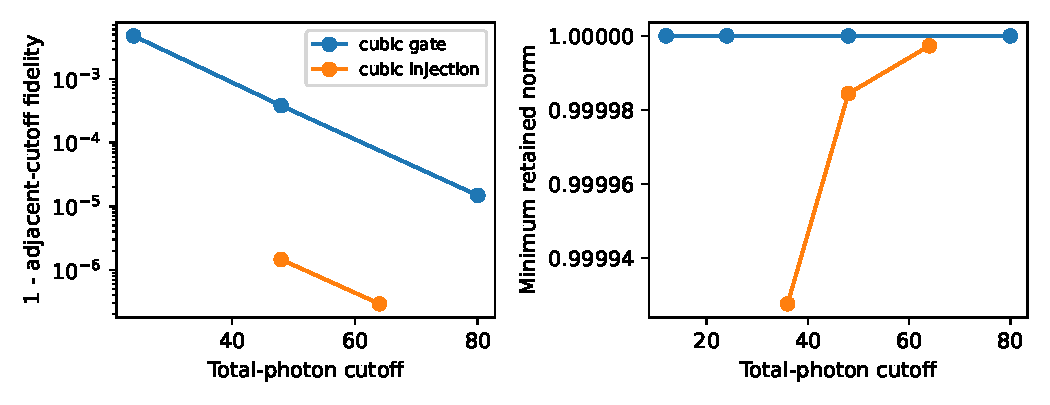
\includegraphics[width=.9\textwidth]{results/non_gaussian_convergence.pdf}
\caption{Cutoff dependence distinguishes a norm-preserving truncated cubic
unitary from converged output physics. The injection trajectory is fixed at
$m=0.4$; its residual norm loss and state change both decrease. Numerical values
and local timings are stored in \texttt{results/non\_gaussian.csv}.}
\end{figure*}

For the strong cubic gate on vacuum, the untruncated theory gives
$\langle p\rangle=\gamma$ and $\langle n\rangle=3\gamma^2/4=0.316875$.
At $c=80$ the recorded mean photon number is approximately $0.316868$;
norm remains one at every tested cutoff. This is numerical evidence on the
specified state, not a uniform bound for stronger gates or arbitrary inputs.
For finite injection the adjacent $48\to64$ fidelity is approximately
$0.999999708$, while the residual envelope in Eq.~\eqref{eq:cubicFilter} remains.

\begin{figure*}[tb]
\centering
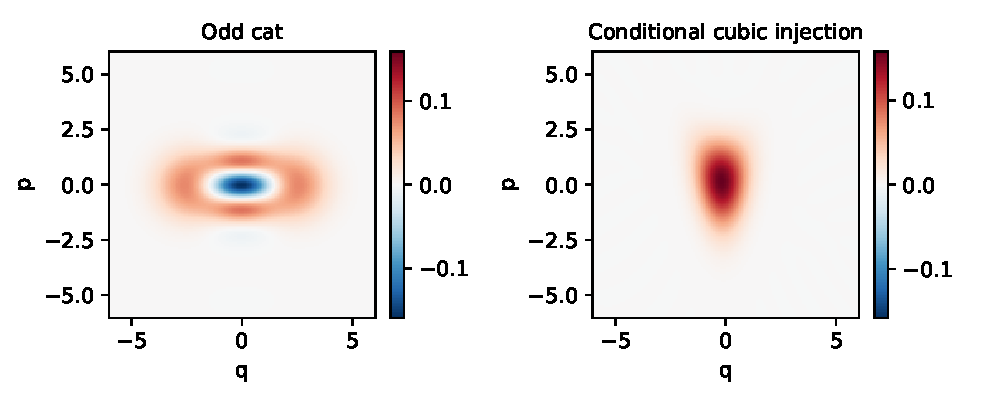
\includegraphics[width=.86\textwidth]{results/non_gaussian_wigner.pdf}
\caption{Single-mode Wigner densities for an odd cat ($\alpha=1.2,c=24$) and
the fixed cubic-injection output ($c=64$). The $161\times161$ window is
$[-6,6]^2$. Captured masses and finite-window negative volumes are saved in
\texttt{results/non\_gaussian\_wigner.json}. These plots are numerical diagnostics;
their finite-grid negativity is not a hardware certification.}
\end{figure*}

The new production modules are \texttt{resources} (cutoff-aware descriptions),
\texttt{capabilities} (preflight), \texttt{fock\_measurements} (conditional
homodyne), \texttt{non\_gaussian} (resource patterns), \texttt{fock\_analysis}
(metrics and Wigner grids), and \texttt{convergence} (branch-aware scans).
The existing commands, states, serialization, simulator and Fock backend are
extended without replacing Gaussian compilation or channel analysis.

\subsection{Noise and present boundaries}

Mixed Fock inputs, Fock loss channels, noisy Fock homodyne, general non-Gaussian
POVMs, dynamic Gaussian-to-Fock switching, GKP decoding and a universal
non-Gaussian compilation path are outside this release. The implemented
operations should be described as experimental non-Gaussian MBQC support.
Gaussian noise support remains thermal attenuation,
$V\mapsto XVX^T+Y$, with local $X=\sqrt\eta\I$ and
$Y=(1-\eta)(2n_{\rm th}+1)\I$. Detector inefficiency is a Gaussian measurement
parameter and finite squeezing is a resource property. Phase diffusion, mode
mismatch and detailed detector hardware are not silently approximated by these
channels.
